\chapter{Outlook}
\section{Conclusions}
This project set out to develop an atom interferometer that could be
suitable for 
inertial navigation. The specific aim was to build a device and demonstrate sensitivity
to horizontal accelerations where gravitational acceleration acts
perpendicularly to the sensitive axis. Requirements for a high
measurement bandwidth and low dead time influenced the development of
the experiment. The project was a team effort in which my particular
tasks were to design, build and programme the computer control systems
and to control the whole complex apparatus through a user interface. I
was also responsible for characterising and understanding the various
sources of noise in the device. 
\par\noindent
The dead time between measurements is reduced by
loading the atoms from a 2D \ac{mot} and through an improved design of
the control software. Using a 2D \ac{mot} reduces the time required to
load a sufficient number of atoms when compared to loading from a
background vapour. The hardware that controls the experiment
regenerates the necessary voltage patterns, removing the need for
additional time to
re-calculate the experimental sequence. This made it possible to load
$10^8$ atoms into the 3D \ac{mot} after \sivalue{100}{\ms}. With a
maximum interrogation time of $2T = $ \sivalue{50}{\ms}, the
interferometer can currently be operated up to a rate of \sivalue{4}{\Hz}, which
corresponds to a duty cycle of 20\%. With further optimisation of the
2D \ac{mot} system, such as increased cooling beam power, it will be
possible to increase the atomic flux and hence increase the experiment
cycling rate. 
\par\noindent
The design of the in-vacuum optical system for the interferometer
light pulses ensures that the fringe visibility is not lost due to
transverse motion of the atoms. Wavefront distortions
of the interferometer light pulses are minimised by not requiring
optical viewports between the Raman laser and the atoms. The beams
are also collimated to a large waist size to reduce dephasing of the
atoms from an intensity gradient. A beam waist of at least
\sivalue{34}{\mm} necessitated an aspheric lens pair in the
collimation optics train. These lenses are not manufactured to the same
optical quality as the triplet lens. It was found that they introduced
an irregular intensity distribution of the laser which led to
dephasing of the atomic states. An improved optical system has been
designed by Shane de Souza, the latest student on this experiment. It
is anticipated that this will improve the wavefront quality for the
interferometer light pulses.
\par\noindent
The sequence of optical and microwave pulses that prepares
atoms in the $\ket{1,0}$ state is very effective at increasing
the population in the $m_F = 0$ state beyond the fraction expected
after an optical molasses. Despite this, there remains a residual
population in the $\ket{1,\pm 1}$ states. These are detected as a
background, which reduces the interferometer fringe contrast. Since
preparing this thesis, the state preparation sequence has been
improved by increasing the polarisation purity of the light driving
the \trans{1}{0} transition. There is now less de-population of the
$\ket{1,0}$ state due to $\pi$-transitions. 
\par\noindent
It has been possible to observe interference with a fringe contrast of
around 5\%. This admittedly low value is likely due to the reasons
stated above. In fact, since reducing the $\ket{1,\pm 1}$ population,
the fringe contrast has increased to around 20\%. Further details of
this can be found in Xiaxi Cheng's PhD thesis~\cite{Cheng2018}.
\par\noindent
The sensitivity to horizontal accelerations was demonstrated by
comparing the interferometer signal in differing levels of vibration
noise. This also highlighted the importance of vibration isolation for
accurate acceleration measurements. A study has been made of a hybrid
system in which the atom interferometer works together with a MEMS
accelerometer. Using this, we have been able to reach a sensitivity to
acceleration of \sivalue{3}{\um\tothe{-2}} after an integration time
of \sivalue{40}{\s}. This will be particularly important in a high-vibration
environment where the classical accelerometer can identify the order
number of the atom interferometer fringe. 
\section{Avenues of Further Research}
Although this work represents the first step towards inertial
navigation using atom interferometry, there is still more to be done.
The bias is one area to study. It is believed that the
interferometer will have exceedingly low bias and that its main role
might be to correct the bias of an associated conventional
accelerometer. This is important as any bias can result in significant
position error at long times. When navigating on the surface of the
Earth, there is a feedback mechanism which partially corrects for bias
and leads to Schuler oscillations~\cite{Schuler1923}. Nevertheless, it
is desirable to have no bias and that seems possible with atom
interferometry. Further work is planned to extend this system to measure accelerations
along 3 axes. This requires a modification of the Raman laser system so
that it can provide enough power from three outputs. It will be
important to have good control over the orientation of the
accelerometer.
\par\noindent
A comparison of the interferometer with conventional
accelerometers will greatly benefit research aimed towards
practical applications of atom interferometry. This has already been
demonstrated in the context of gravimeters~\cite{Farah2014,Gillot2014}, where a
mobile atomic system has demonstrated greater insensitivity to
vibration noise and better short-term stability than the
state-of-the-art classical counterpart. Additionally, this interferometer has
yet to be tested outside of a laboratory environment. As a first step
in that direction, it was demonstrated at the UK National Quantum
Technologies Showcase in November $2018$ in the Queen Elizabeth II
conference centre (see~\FigureRef{fig:qe2}), where it operated in a normal room in the
presence of 800 people and a large fluctuating ambient magnetic field. A recent
experiment has investigated the bias stability of a hybrid sensor in a
simulated harsh environment~\cite{Cheiney2018}.   
\begin{figure}[htpb]
  \centering
  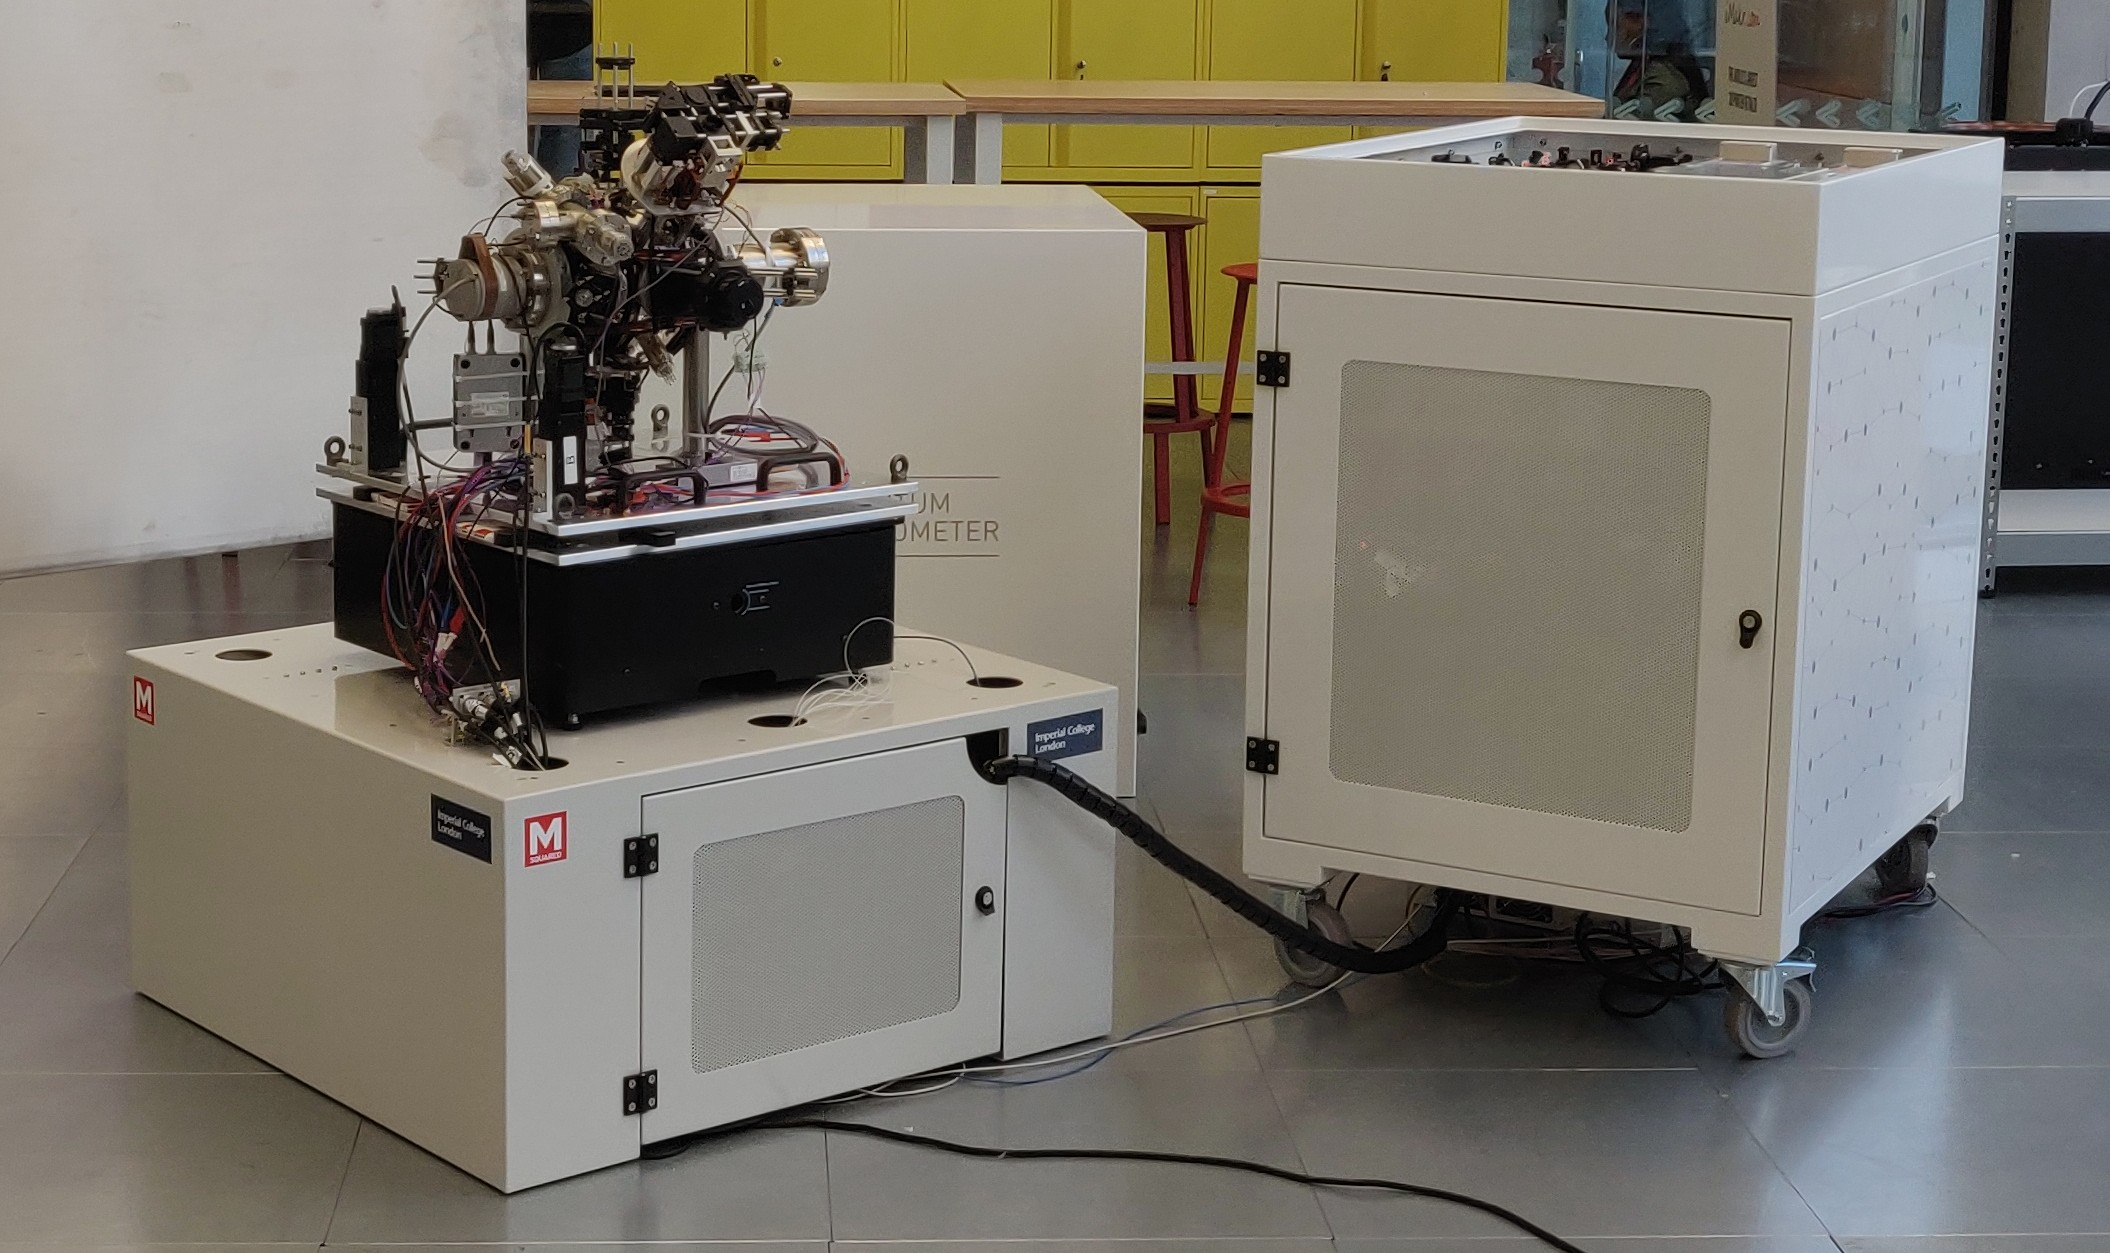
\includegraphics[width=0.8\linewidth]{qe2.jpg}
  \caption{Demonstration of the atom interferometer as a mobile sensor
  of a range of horizontal accelerations at the UK National Quantum
Technologies Showcase in November 2018.}
\label{fig:qe2}
\end{figure}
\section{Concluding Remarks}
The application of newly understood physics has often led to the
development of more advanced technology. In turn, this has contributed
to further progress in scientific disciplines, and society in general.
This describes well the present effort to use matter-wave
interferometry for inertial sensing. There already exists a significant
body of research that demonstrates the technical feasibility of
measuring inertial forces using cold atomic systems. In addition, the
practical requirements for navigation have served to identify a need
for the unique benefits of atom interferometers. The work presented
in this thesis has helped to address this need. It is anticipated that
the application of quantum mechanics to technology will
bring practical benefits as well as enable a deeper understanding of
physical phenomena.
\let\clearpage\relax
